% Generated on 2023-11-22 18:14:05 by gEcon ver. 1.2.1 (2023-01-18)
% http://gecon.r-forge.r-project.org/

% Model name: RSW_RP_PERS

\section{Steady-state values}


\begin{tabular}{c|c|}
  & Steady-state value\\
\hline
${e\!t\!a\!p\!i}$ & 1 \\
${i\!H}$ & -0.0207 \\
${i\!L}$ & -1.9792 \\
$\lambda^{\mathrm{HIGHREGIME}^{\mathrm{1}}}$ & 0.0027 \\
$\lambda^{\mathrm{HIGHREGIME}^{\mathrm{2}}}$ & 0 \\
$\lambda^{\mathrm{LOWREGIME}^{\mathrm{1}}}$ & -0.0082 \\
$\lambda^{\mathrm{LOWREGIME}^{\mathrm{2}}}$ & 0 \\
$\lambda^{\mathrm{HIGHREGIME}^{\mathrm{piH}^{\mathrm{lag}^{\mathrm{1}}}}}$ & 0.0021 \\
$\lambda^{\mathrm{LOWREGIME}^{\mathrm{piL}^{\mathrm{lag}^{\mathrm{1}}}}}$ & -0.0064 \\
${p\!i\!H}$ & 0 \\
${p\!i\!L}$ & -1.9999 \\
${p\!i\!H}^{\mathrm{lag}^{\mathrm{1}}}$ & 0 \\
${p\!i\!L}^{\mathrm{lag}^{\mathrm{1}}}$ & -1.9999 \\
${y\!H}$ & 0.0161 \\
${y\!L}$ & -0.0484 \\
${U\!H}$ & -0.0019 \\
${U\!L}$ & -0.0034 \\
\hline
\end{tabular}


\section{The solution of the 1st order perturbation}

\subsection*{Matrix $P$}

$$\bordermatrix{
~ & {e\!t\!a\!p\!i}_{t-1} & {i\!H}_{t-1} & {i\!L}_{t-1} & {p\!i\!H}_{t-1} & {p\!i\!L}_{t-1} & {p\!i\!H}^{\mathrm{lag}^{\mathrm{1}}}_{t-1} & {p\!i\!L}^{\mathrm{lag}^{\mathrm{1}}}_{t-1} & {y\!H}_{t-1} & {y\!L}_{t-1} \cr
{e\!t\!a\!p\!i}_{t} & 0.95 & 0 & 0 & 0 & 0 & 0 & 0 & 0 & 0 \cr
{i\!H}_{t} & -8109.1373 & -7.0346 & 7.121 & 5967.7856 & -163.955 & -5522.7592 & 132.0006 & -32.7973 & 1.1574 \cr
{i\!L}_{t} & -86.4454 & 0.0008 & -7.1 & -0.8717 & 127.6919 & 0.7026 & -117.9682 & 0.0041 & -1.0523 \cr
{p\!i\!H}_{t} & -5.05 & 0 & 0 & 5.102 & -0.1041 & -4.0816 & 0.0833 & -0.0202 & 0.0006 \cr
{p\!i\!L}_{t} & -2.5512 & 0 & 0 & -0.026 & 5.1541 & 0.0208 & -4.1233 & 0.0001 & -0.0307 \cr
{p\!i\!H}^{\mathrm{lag}^{\mathrm{1}}}_{t} & 0 & 0 & 0 & 1 & 0 & 0 & 0 & 0 & 0 \cr
{p\!i\!L}^{\mathrm{lag}^{\mathrm{1}}}_{t} & 0 & 0 & 0 & 0 & 1 & 0 & 0 & 0 & 0 \cr
{y\!H}_{t} & 314.385 & 1.3009 & -1.2573 & -317.6261 & 6.4817 & 254.1009 & -5.1854 & 2.2679 & -0.0693 \cr
{y\!L}_{t} & 105.5163 & -0.0044 & 41.3501 & 1.0767 & -213.1706 & -0.8614 & 170.5364 & -0.0077 & 2.2807 \cr
}$$

\subsection*{Matrix $Q$}

$$\bordermatrix{
~ & \epsilon^{\pi} \cr
{e\!t\!a\!p\!i} & 1 \cr
{i\!H} & -1355.9943 \cr
{i\!L} & -14.3033 \cr
{p\!i\!H} & 0 \cr
{p\!i\!L} & 0 \cr
{p\!i\!H}^{\mathrm{lag}^{\mathrm{1}}} & 0 \cr
{p\!i\!L}^{\mathrm{lag}^{\mathrm{1}}} & 0 \cr
{y\!H} & 0 \cr
{y\!L} & 0 \cr
}$$

\subsection*{Matrix $R$}

$$\bordermatrix{
~ & {e\!t\!a\!p\!i}_{t-1} & {i\!H}_{t-1} & {i\!L}_{t-1} & {p\!i\!H}_{t-1} & {p\!i\!L}_{t-1} & {p\!i\!H}^{\mathrm{lag}^{\mathrm{1}}}_{t-1} & {p\!i\!L}^{\mathrm{lag}^{\mathrm{1}}}_{t-1} & {y\!H}_{t-1} & {y\!L}_{t-1} \cr
\lambda^{\mathrm{HIGHREGIME}^{\mathrm{1}}}_{t} & -753292.161 & -553.6177 & 1083.6189 & 579732.8846 & -26093.2637 & -532367.5156 & 22299.2884 & -3064.8326 & 192.6019 \cr
\lambda^{\mathrm{HIGHREGIME}^{\mathrm{2}}}_{t} & 83.0178 & 0.0625 & -0.1218 & -63.5359 & 2.8921 & 58.4868 & -2.4731 & 0.338 & -0.0214 \cr
\lambda^{\mathrm{LOWREGIME}^{\mathrm{1}}}_{t} & -260586.2362 & 3.8616 & -18155.8024 & -4425.8716 & 402055.8445 & 3782.3863 & -368655.4108 & 21.7194 & -3190.0187 \cr
\lambda^{\mathrm{LOWREGIME}^{\mathrm{2}}}_{t} & 85.5602 & -0.0013 & 6.1044 & 1.4612 & -131.2999 & -1.2495 & 120.6755 & -0.0072 & 1.0482 \cr
\lambda^{\mathrm{HIGHREGIME}^{\mathrm{piH}^{\mathrm{lag}^{\mathrm{1}}}}}_{t} & -124226.593 & -92.4713 & 181.4621 & 94997.2441 & -4332.2135 & -87486.2434 & 3704.9419 & -504.8164 & 32.0348 \cr
\lambda^{\mathrm{LOWREGIME}^{\mathrm{piL}^{\mathrm{lag}^{\mathrm{1}}}}}_{t} & -42534.3851 & 0.6399 & -3000.8484 & -727.1404 & 65221.6942 & 621.8577 & -59969.5328 & 3.5747 & -520.0821 \cr
{U\!H}_{t} & 13.9888 & 0 & 0.0744 & -0.2786 & -1.9913 & 1.1001 & 1.7864 & 0.0054 & 0.0151 \cr
{U\!L}_{t} & -34.3598 & 0 & 0.0008 & 0.0022 & 1.0317 & -0.0011 & -3.8714 & 0 & -0.0288 \cr
}$$

\subsection*{Matrix $S$}

$$\bordermatrix{
~ & \epsilon^{\pi} \cr
\lambda^{\mathrm{HIGHREGIME}^{\mathrm{1}}} & -107127.1888 \cr
\lambda^{\mathrm{HIGHREGIME}^{\mathrm{2}}} & 12.0579 \cr
\lambda^{\mathrm{LOWREGIME}^{\mathrm{1}}} & -36724.1369 \cr
\lambda^{\mathrm{LOWREGIME}^{\mathrm{2}}} & 12.3099 \cr
\lambda^{\mathrm{HIGHREGIME}^{\mathrm{piH}^{\mathrm{lag}^{\mathrm{1}}}}} & -18088.9945 \cr
\lambda^{\mathrm{LOWREGIME}^{\mathrm{piL}^{\mathrm{lag}^{\mathrm{1}}}}} & -6134.7786 \cr
{U\!H} & 12.1022 \cr
{U\!L} & -33.6196 \cr
}$$


\section{Model statistics}

\subsection{Basic statistics}

\begin{tabular}{c|c|c|c|c|}
  & Steady-state value & Std. dev. & Variance & Loglin\\
\hline
${e\!t\!a\!p\!i}$ & 1 & 0.1303 & 0.017 & Y    \\
${i\!H}$ & -0.0207 & 191.9455 & 36843.0774 & Y    \\
${i\!L}$ & -1.9792 & 2.0269 & 4.1082 & Y    \\
$\lambda^{\mathrm{HIGHREGIME}^{\mathrm{1}}}$ & 0.0027 & 10335.6952 & 106826594.4718 & Y    \\
$\lambda^{\mathrm{HIGHREGIME}^{\mathrm{2}}}$ & 0 & 1.1627 & 1.3519 & N    \\
$\lambda^{\mathrm{LOWREGIME}^{\mathrm{1}}}$ & -0.0082 & 3542.6886 & 12550642.2407 & Y    \\
$\lambda^{\mathrm{LOWREGIME}^{\mathrm{2}}}$ & 0 & 1.187 & 1.409 & N    \\
$\lambda^{\mathrm{HIGHREGIME}^{\mathrm{piH}^{\mathrm{lag}^{\mathrm{1}}}}}$ & 0.0021 & 1737.9387 & 3020431.0324 & Y    \\
$\lambda^{\mathrm{LOWREGIME}^{\mathrm{piL}^{\mathrm{lag}^{\mathrm{1}}}}}$ & -0.0064 & 589.4457 & 347446.2292 & Y    \\
${p\!i\!H}$ & 0 & 0.5011 & 0.2511 & N    \\
${p\!i\!L}$ & -1.9999 & 0.2531 & 0.0641 & Y    \\
${p\!i\!H}^{\mathrm{lag}^{\mathrm{1}}}$ & 0 & 0.5011 & 0.2511 & N    \\
${p\!i\!L}^{\mathrm{lag}^{\mathrm{1}}}$ & -1.9999 & 0.2531 & 0.0641 & Y    \\
${y\!H}$ & 0.0161 & 144.362 & 20840.3795 & Y    \\
${y\!L}$ & -0.0484 & 48.4503 & 2347.4304 & Y    \\
${U\!H}$ & -0.0019 & 1.5297 & 2.3399 & Y    \\
${U\!L}$ & -0.0034 & 4.2417 & 17.9917 & Y    \\
\hline
\end{tabular}


\subsection{Correlation matrix}

\begin{tabular}{c|ccccccccccccccccc|}
  & ${e\!t\!a\!p\!i}$ & ${i\!H}$ & ${i\!L}$ & $\lambda^{\mathrm{HIGHREGIME}^{\mathrm{1}}}$ & $\lambda^{\mathrm{HIGHREGIME}^{\mathrm{2}}}$ & $\lambda^{\mathrm{LOWREGIME}^{\mathrm{1}}}$ & $\lambda^{\mathrm{LOWREGIME}^{\mathrm{2}}}$ & $\lambda^{\mathrm{HIGHREGIME}^{\mathrm{piH}^{\mathrm{lag}^{\mathrm{1}}}}}$ & $\lambda^{\mathrm{LOWREGIME}^{\mathrm{piL}^{\mathrm{lag}^{\mathrm{1}}}}}$ & ${p\!i\!H}$ & ${p\!i\!L}$ & ${p\!i\!H}^{\mathrm{lag}^{\mathrm{1}}}$ & ${p\!i\!L}^{\mathrm{lag}^{\mathrm{1}}}$ & ${y\!H}$ & ${y\!L}$ & ${U\!H}$ & ${U\!L}$\\
\hline
${e\!t\!a\!p\!i}$ & 1 & -0.117 & -0.116 & -0.499 & 0.436 & -0.498 & 0.436 & -0.46 & -0.46 & -0.452 & -0.452 & -0.361 & -0.361 & -0.275 & -0.274 & 0.939 & -0.977 \\
${i\!H}$ &  & 1 & 1 & 0.593 & -0.716 & 0.595 & -0.716 & 0.657 & 0.657 & -0.667 & -0.667 & 0.149 & 0.149 & -0.744 & -0.743 & -0.003 & 0.049 \\
${i\!L}$ &  &  & 1 & 0.592 & -0.715 & 0.594 & -0.715 & 0.656 & 0.657 & -0.667 & -0.667 & 0.15 & 0.15 & -0.744 & -0.744 & -0.002 & 0.048 \\
$\lambda^{\mathrm{HIGHREGIME}^{\mathrm{1}}}$ &  &  &  & 1 & -0.986 & 1 & -0.986 & 0.995 & 0.995 & 0.066 & 0.066 & -0.097 & -0.097 & 0.068 & 0.069 & -0.559 & 0.541 \\
$\lambda^{\mathrm{HIGHREGIME}^{\mathrm{2}}}$ &  &  &  &  & 1 & -0.986 & 1 & -0.997 & -0.997 & 0.097 & 0.097 & 0.092 & 0.092 & 0.085 & 0.084 & 0.476 & -0.466 \\
$\lambda^{\mathrm{LOWREGIME}^{\mathrm{1}}}$ &  &  &  &  &  & 1 & -0.986 & 0.995 & 0.995 & 0.064 & 0.064 & -0.097 & -0.097 & 0.067 & 0.067 & -0.559 & 0.541 \\
$\lambda^{\mathrm{LOWREGIME}^{\mathrm{2}}}$ &  &  &  &  &  &  & 1 & -0.997 & -0.997 & 0.097 & 0.097 & 0.092 & 0.092 & 0.085 & 0.084 & 0.476 & -0.466 \\
$\lambda^{\mathrm{HIGHREGIME}^{\mathrm{piH}^{\mathrm{lag}^{\mathrm{1}}}}}$ &  &  &  &  &  &  &  & 1 & 1 & -0.032 & -0.032 & -0.126 & -0.126 & -0.002 & -0.002 & -0.52 & 0.502 \\
$\lambda^{\mathrm{LOWREGIME}^{\mathrm{piL}^{\mathrm{lag}^{\mathrm{1}}}}}$ &  &  &  &  &  &  &  &  & 1 & -0.033 & -0.033 & -0.126 & -0.126 & -0.003 & -0.003 & -0.52 & 0.502 \\
${p\!i\!H}$ &  &  &  &  &  &  &  &  &  & 1 & 1 & 0.226 & 0.226 & 0.782 & 0.781 & -0.481 & 0.473 \\
${p\!i\!L}$ &  &  &  &  &  &  &  &  &  &  & 1 & 0.225 & 0.225 & 0.782 & 0.782 & -0.482 & 0.473 \\
${p\!i\!H}^{\mathrm{lag}^{\mathrm{1}}}$ &  &  &  &  &  &  &  &  &  &  &  & 1 & 1 & -0.408 & -0.41 & -0.03 & 0.159 \\
${p\!i\!L}^{\mathrm{lag}^{\mathrm{1}}}$ &  &  &  &  &  &  &  &  &  &  &  &  & 1 & -0.408 & -0.41 & -0.03 & 0.159 \\
${y\!H}$ &  &  &  &  &  &  &  &  &  &  &  &  &  & 1 & 1 & -0.508 & 0.422 \\
${y\!L}$ &  &  &  &  &  &  &  &  &  &  &  &  &  &  & 1 & -0.507 & 0.421 \\
${U\!H}$ &  &  &  &  &  &  &  &  &  &  &  &  &  &  &  & 1 & -0.991 \\
${U\!L}$ &  &  &  &  &  &  &  &  &  &  &  &  &  &  &  &  & 1 \\
\hline
\end{tabular}


\subsection{Cross correlations with the reference variable (${i\!H}$)}

\begin{tabular}{c|c|c|c|c|c|c|c|c|c|c|c|c|}
  & $\sigma[\cdot]$ rel. to $\sigma[{i\!H}]$ & ${i\!H}_{t-5}$ & ${i\!H}_{t-4}$ & ${i\!H}_{t-3}$ & ${i\!H}_{t-2}$ & ${i\!H}_{t-1}$ & ${i\!H}_{t}$ & ${i\!H}_{t+1}$ & ${i\!H}_{t+2}$ & ${i\!H}_{t+3}$ & ${i\!H}_{t+4}$ & ${i\!H}_{t+5}$\\
\hline
${e\!t\!a\!p\!i}_{t}$ & 0.001 & 0.042 & 0.036 & -0.019 & -0.113 & 0.435 & -0.117 & -0.098 & -0.081 & -0.065 & -0.051 & -0.038 \\
${i\!H}_{t}$ & 1 & -0.002 & 0.009 & 0.043 & 0.04 & -0.576 & 1 & -0.576 & 0.04 & 0.043 & 0.009 & -0.002 \\
${i\!L}_{t}$ & 0.011 & -0.002 & 0.009 & 0.043 & 0.04 & -0.575 & 1 & -0.577 & 0.04 & 0.043 & 0.009 & -0.002 \\
$\lambda^{\mathrm{HIGHREGIME}^{\mathrm{1}}}_{t}$ & 53.847 & -0.015 & 0.003 & 0.073 & 0.141 & -0.71 & 0.593 & 0.093 & -0.007 & -0.021 & -0.019 & -0.016 \\
$\lambda^{\mathrm{HIGHREGIME}^{\mathrm{2}}}_{t}$ & 0.006 & 0.013 & -0.005 & -0.072 & -0.129 & 0.733 & -0.716 & 0.017 & 0.017 & 0.016 & 0.015 & 0.014 \\
$\lambda^{\mathrm{LOWREGIME}^{\mathrm{1}}}_{t}$ & 18.457 & -0.015 & 0.003 & 0.073 & 0.141 & -0.71 & 0.595 & 0.092 & -0.008 & -0.021 & -0.019 & -0.016 \\
$\lambda^{\mathrm{LOWREGIME}^{\mathrm{2}}}_{t}$ & 0.006 & 0.013 & -0.005 & -0.072 & -0.129 & 0.733 & -0.716 & 0.017 & 0.017 & 0.016 & 0.015 & 0.014 \\
$\lambda^{\mathrm{HIGHREGIME}^{\mathrm{piH}^{\mathrm{lag}^{\mathrm{1}}}}}_{t}$ & 9.054 & -0.014 & 0.004 & 0.073 & 0.135 & -0.728 & 0.657 & 0.055 & -0.03 & -0.024 & -0.016 & -0.013 \\
$\lambda^{\mathrm{LOWREGIME}^{\mathrm{piL}^{\mathrm{lag}^{\mathrm{1}}}}}_{t}$ & 3.071 & -0.014 & 0.004 & 0.073 & 0.135 & -0.728 & 0.657 & 0.054 & -0.03 & -0.024 & -0.016 & -0.013 \\
${p\!i\!H}_{t}$ & 0.003 & -0.017 & -0.017 & 0 & 0.071 & 0.149 & -0.667 & 0.466 & 0.177 & 0.016 & -0.021 & -0.023 \\
${p\!i\!L}_{t}$ & 0.001 & -0.017 & -0.017 & 0 & 0.071 & 0.149 & -0.667 & 0.466 & 0.176 & 0.016 & -0.02 & -0.023 \\
${p\!i\!H}^{\mathrm{lag}^{\mathrm{1}}}_{t}$ & 0.003 & -0.014 & -0.017 & -0.017 & 0 & 0.071 & 0.149 & -0.667 & 0.466 & 0.177 & 0.016 & -0.021 \\
${p\!i\!L}^{\mathrm{lag}^{\mathrm{1}}}_{t}$ & 0.001 & -0.014 & -0.017 & -0.017 & 0 & 0.071 & 0.149 & -0.667 & 0.466 & 0.176 & 0.016 & -0.02 \\
${y\!H}_{t}$ & 0.752 & -0.012 & -0.011 & 0.004 & 0.062 & 0.098 & -0.744 & 0.868 & -0.156 & -0.091 & -0.014 & 0.007 \\
${y\!L}_{t}$ & 0.252 & -0.012 & -0.011 & 0.004 & 0.062 & 0.098 & -0.743 & 0.868 & -0.157 & -0.091 & -0.014 & 0.007 \\
${U\!H}_{t}$ & 0.008 & 0.04 & 0.033 & -0.026 & -0.124 & 0.46 & -0.003 & -0.389 & 0.067 & -0.004 & -0.044 & -0.044 \\
${U\!L}_{t}$ & 0.022 & -0.041 & -0.035 & 0.023 & 0.121 & -0.457 & 0.049 & 0.28 & -0.012 & 0.028 & 0.048 & 0.043 \\
\hline
\end{tabular}


\subsection{Autocorrelations}

\begin{tabular}{c|ccccc|}
  & Lag 1 & Lag 2 & Lag 3 & Lag 4 & Lag 5\\
\hline
${e\!t\!a\!p\!i}$ & 0.713 & 0.471 & 0.271 & 0.11 & -0.016 \\
${i\!H}$ & -0.576 & 0.04 & 0.043 & 0.009 & -0.002 \\
${i\!L}$ & -0.576 & 0.04 & 0.043 & 0.009 & -0.002 \\
$\lambda^{\mathrm{HIGHREGIME}^{\mathrm{1}}}$ & 0.08 & -0.085 & -0.096 & -0.085 & -0.074 \\
$\lambda^{\mathrm{HIGHREGIME}^{\mathrm{2}}}$ & -0.074 & -0.071 & -0.066 & -0.06 & -0.054 \\
$\lambda^{\mathrm{LOWREGIME}^{\mathrm{1}}}$ & 0.079 & -0.085 & -0.096 & -0.085 & -0.074 \\
$\lambda^{\mathrm{LOWREGIME}^{\mathrm{2}}}$ & -0.074 & -0.071 & -0.066 & -0.06 & -0.054 \\
$\lambda^{\mathrm{HIGHREGIME}^{\mathrm{piH}^{\mathrm{lag}^{\mathrm{1}}}}}$ & -0.005 & -0.109 & -0.083 & -0.065 & -0.055 \\
$\lambda^{\mathrm{LOWREGIME}^{\mathrm{piL}^{\mathrm{lag}^{\mathrm{1}}}}}$ & -0.006 & -0.109 & -0.083 & -0.065 & -0.056 \\
${p\!i\!H}$ & 0.226 & -0.072 & -0.122 & -0.114 & -0.1 \\
${p\!i\!L}$ & 0.225 & -0.072 & -0.122 & -0.114 & -0.1 \\
${p\!i\!H}^{\mathrm{lag}^{\mathrm{1}}}$ & 0.226 & -0.072 & -0.122 & -0.114 & -0.1 \\
${p\!i\!L}^{\mathrm{lag}^{\mathrm{1}}}$ & 0.225 & -0.072 & -0.122 & -0.114 & -0.1 \\
${y\!H}$ & -0.317 & -0.138 & -0.011 & 0.015 & 0.012 \\
${y\!L}$ & -0.317 & -0.138 & -0.011 & 0.015 & 0.012 \\
${U\!H}$ & 0.566 & 0.206 & 0.258 & 0.182 & 0.064 \\
${U\!L}$ & 0.644 & 0.326 & 0.279 & 0.164 & 0.037 \\
\hline
\end{tabular}



\pagebreak

\section{Impulse response functions}

\begin{figure}[h]
\begin{minipage}{0.5\textwidth}
\vspace*{-3em}
\centering
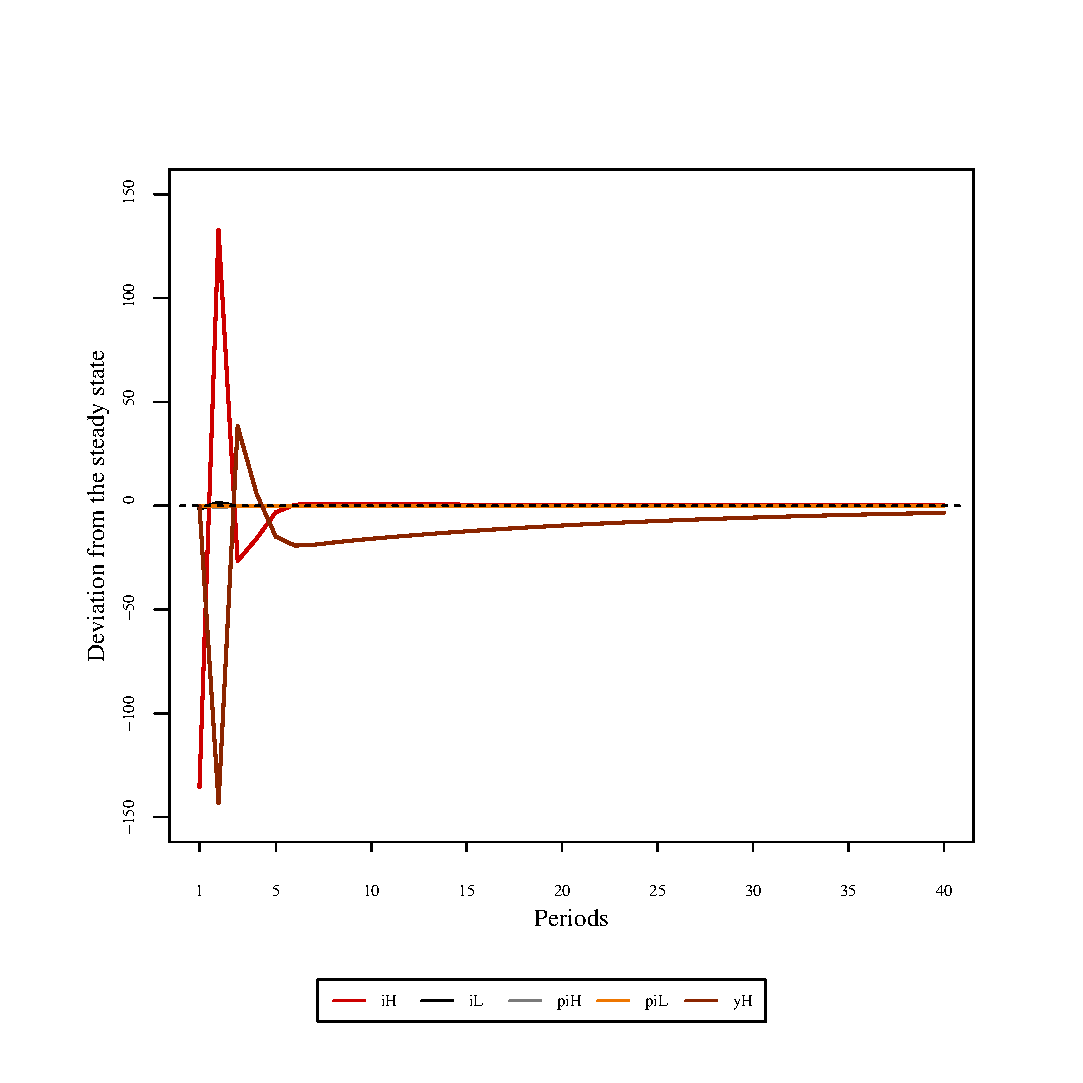
\includegraphics[width=0.99\textwidth, scale=0.55]{plots/plot_47.eps}
\caption{Impulse responses (${i\!H}, {i\!L}, {p\!i\!H}, {p\!i\!L}, {y\!H}$) to $\epsilon^{\pi}$ shock}
\end{minipage}
\begin{minipage}{0.5\textwidth}
\vspace*{-3em}
\centering
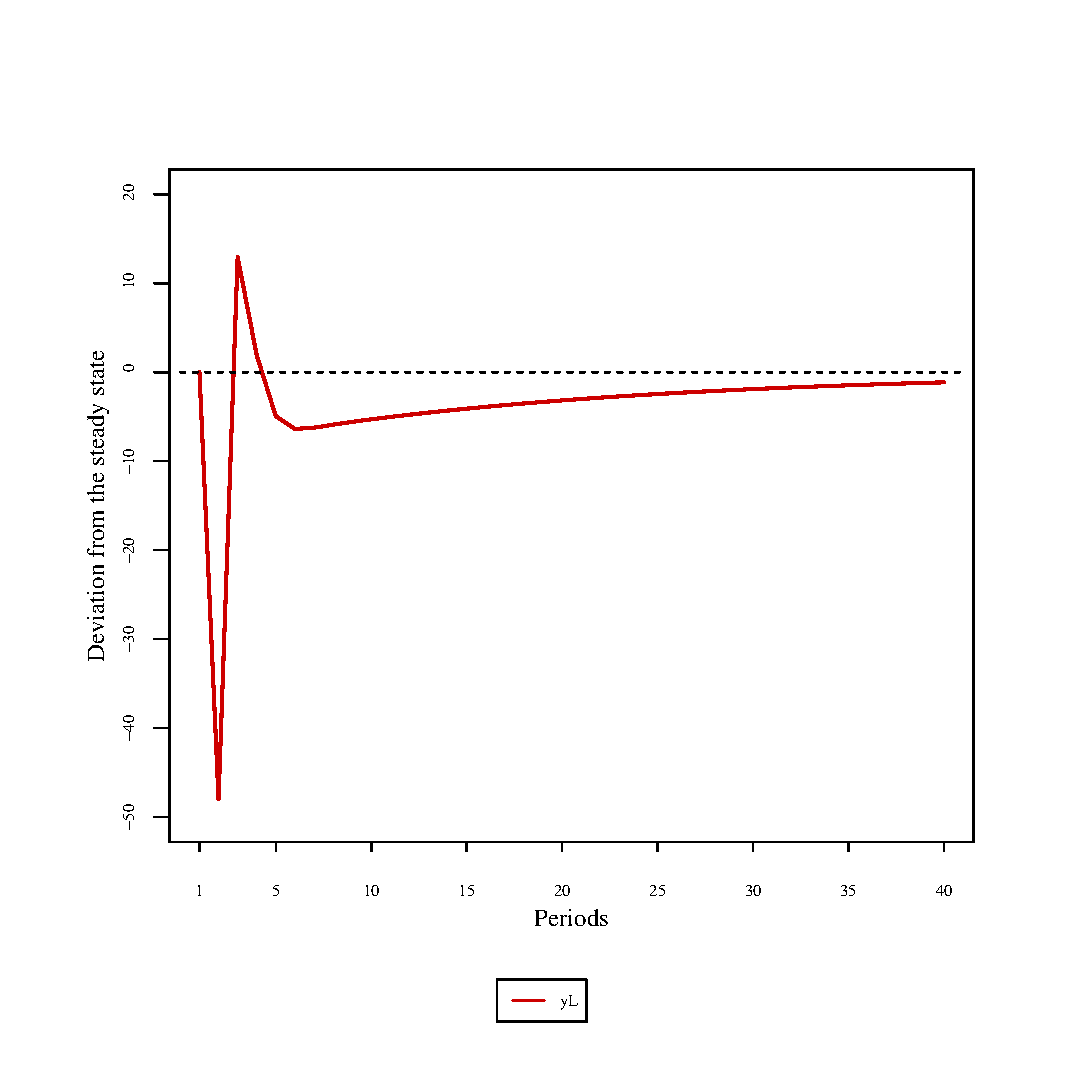
\includegraphics[width=0.99\textwidth, scale=0.55]{plots/plot_48.eps}
\caption{Impulse response (${y\!L}$) to $\epsilon^{\pi}$ shock}
\end{minipage}
\end{figure}


